\section{System Design}
We first present our system architecture and then dive into each component to justify our design choices.

\begin{figure}[t]
\centering
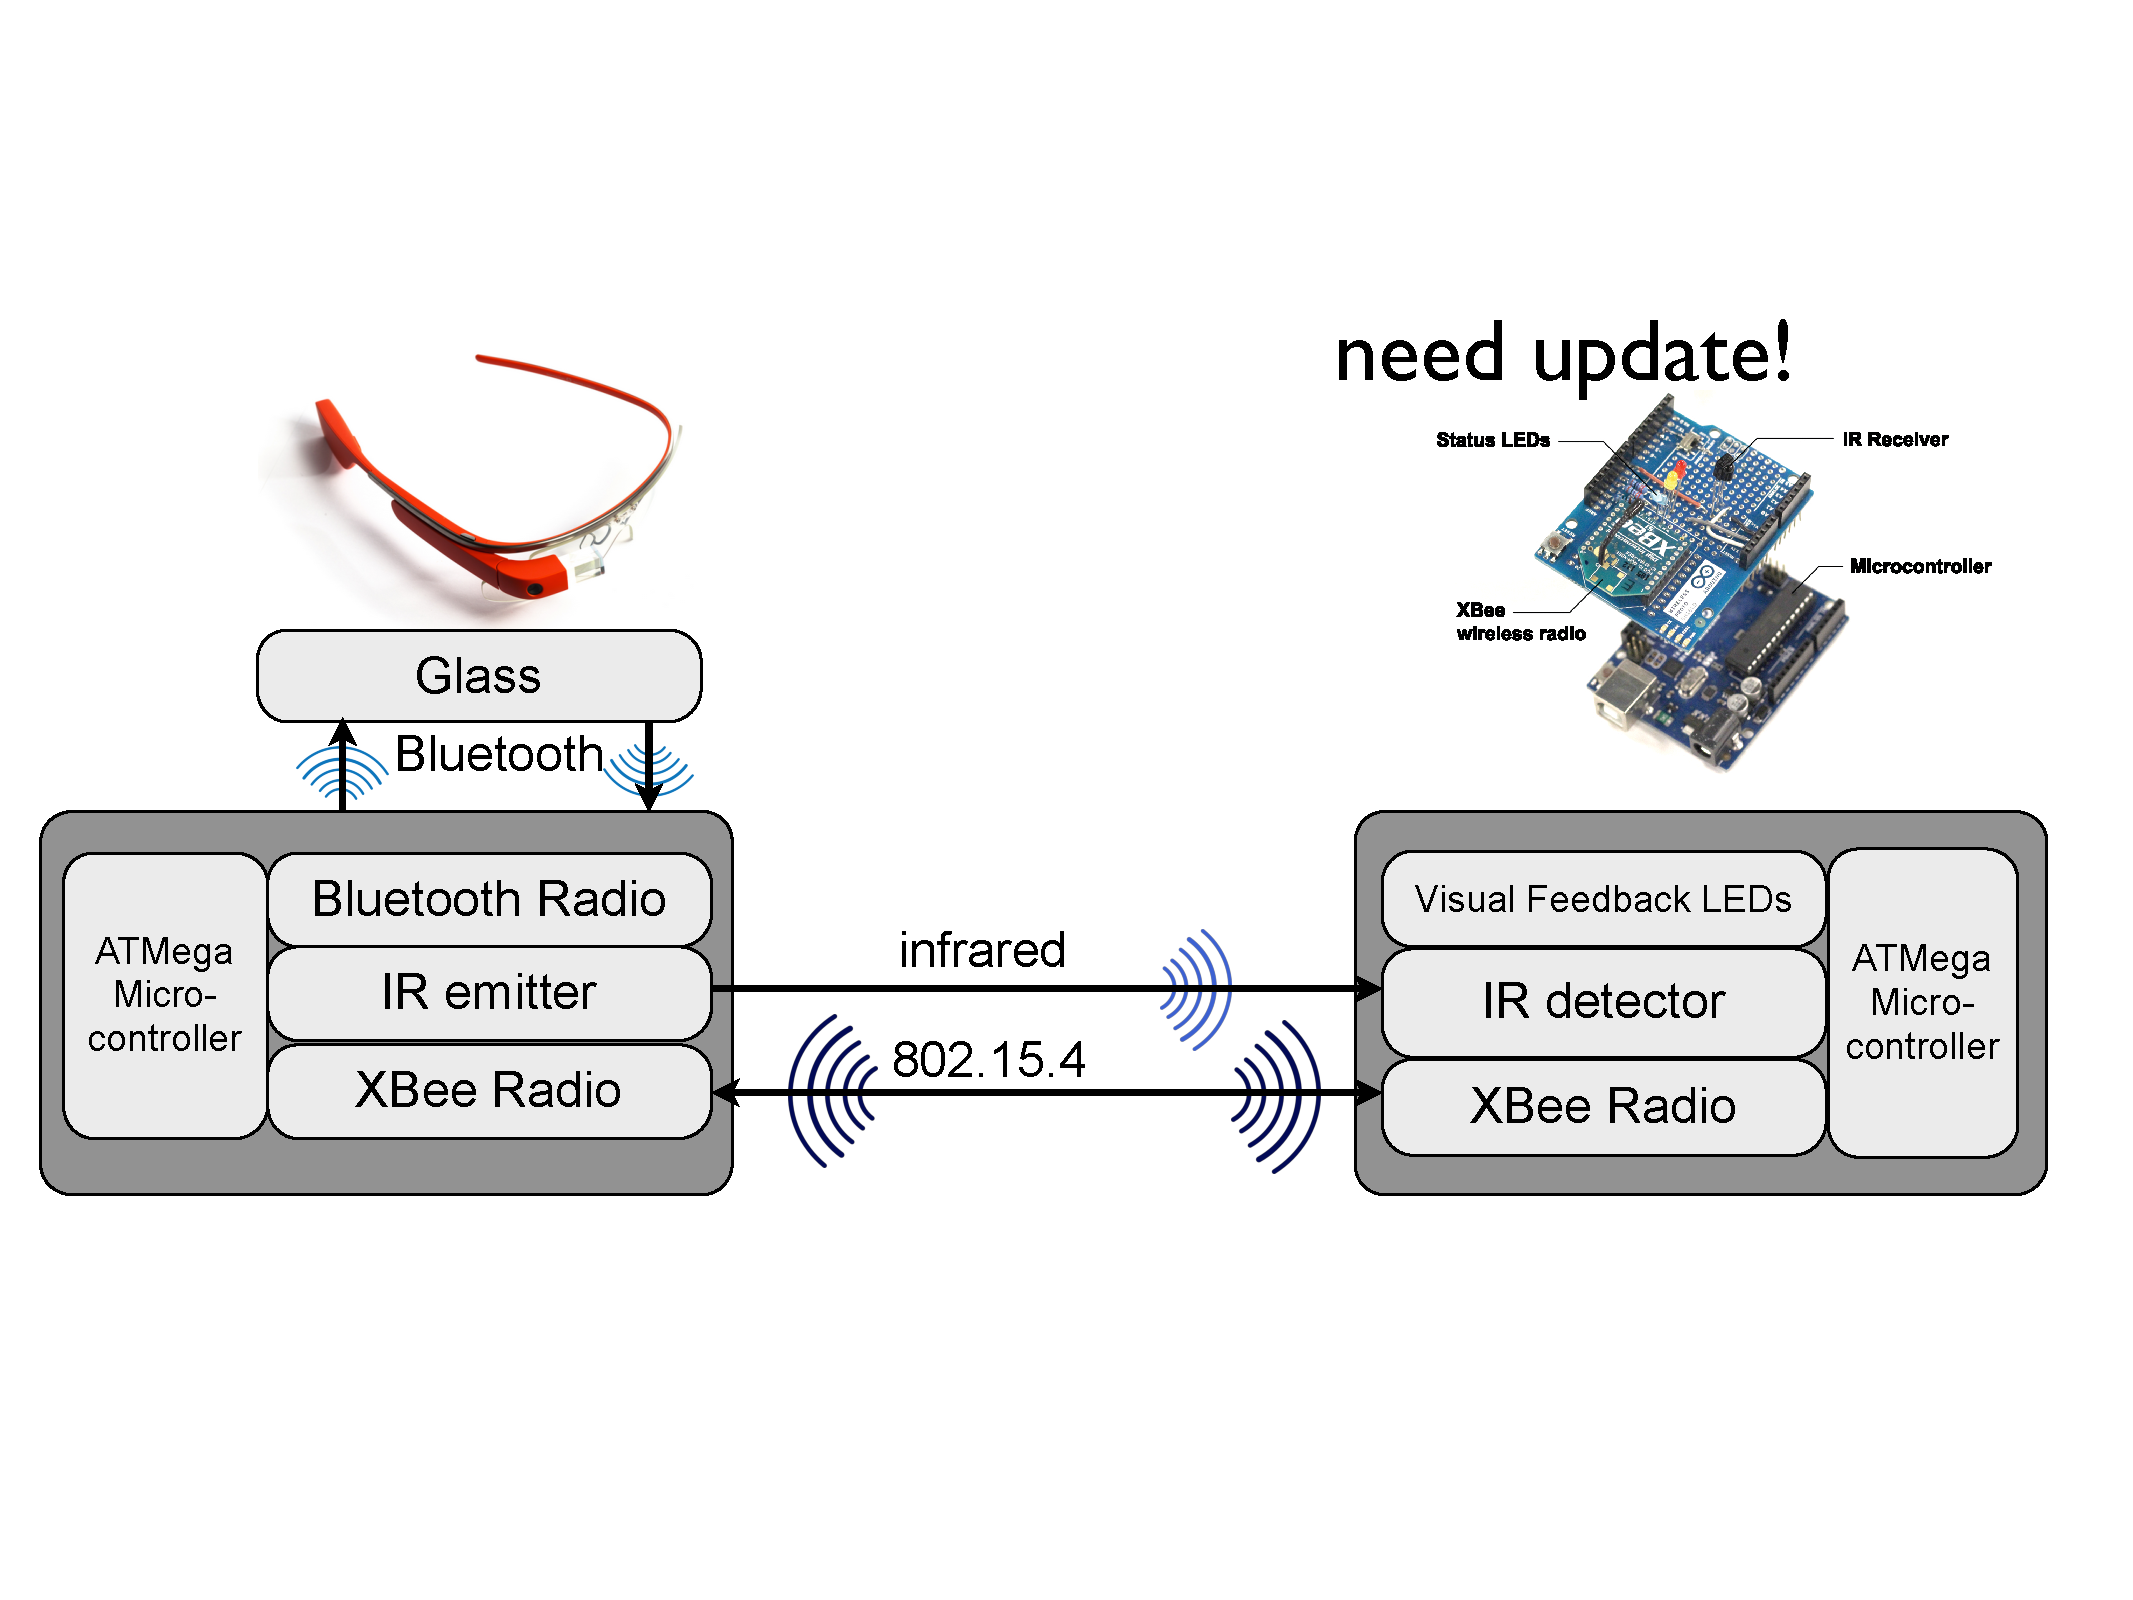
\includegraphics[width=0.9\columnwidth]{figures/architecture.pdf}
\caption{In our system architecture, targeting is captured by IR signal but the confirmation is over 802.15.4 radio. In the research prototype, users have to carry an additional microcontroller board that marshals messages between Google Glass' Bluetooth radio and the IR/802.15.4 interface. But our customized hardware can be also integrated into the wearable device.}
\label{fig:architecture}
\end{figure}

%% IR is a proper choice.
{\bf Area Beam Cursor:} To achieve area selection, our design focuses on using IR signals to detect the general head orientation in physical space. Each selectable target is equipped with IR receivers. We choose IR for a couple of reasons:
\begin{itemize}
\item The signal characteristics of IR makes it suitable for directional area selection. In general, IR covers a viewing angle of $20^\circ$ of viewing angle (though a wider range is avaialble in the market). This leads to a cone shape-like area coverage and can be well-aligned with users' line of sight. 
\item IR has been extensively used for remote control. The emitters and receivers are cheap to manufacture and easy to integrate.
\end{itemize}

%% We have chosen to use Google Glass.
{\bf Head-worn Computing Device:} We use Google Glass among the available COTS head-worn devices because it's easy to program (Android platform) and also light-weight for everyday use.

%% the following is commented out because it's hard to have it while we describe the iterative design procedure
%% We are interested in sensing two things: 1) IR communication and 2) IR intensity. Common IR receivers have automatic gain control built in and hide received signal strength. We therefore add an IR intensity sensor. In a commercial application, a single sensor that both decodes and reports RSSI could be designed.

{\bf Wireless communication:} Though there is a wide range of radios available for wireless communication, we made the choice of 802.15.4 and ZigBee protocol because it is specifically for mesh network and the nice integration with Arduino platform. However, for now Google Glass only supports WiFi and Bluetooth. We have to add a Bluetooth modem to bridge Glass and the rest of the system. \footnote{This is a compromise now, and we are planning to migrate the entire system to Bluetooth Low Energy (BLE) once Google upgrades the Glass software to Android 4.4+. The prototype now suffice our demand to study head orientation-based target selection.}
 
{\bf Visual Feedback from the environment:} Each target is equipped with multiple LEDs and these LEDs are used for visual feedback during the target selection process. 

\ben{discussion on the choices of each}.
This architecture was chosen for reasons of expediency and we do not claim optimality for our design decisions. Future head-mounted devices could clearly integrate IR emitters; the choice of local wireless technology could also change. In particular, one could substitute WiFi modules or design an all-Bluetooth network.


%%% Local Variables: 
%%% mode: latex
%%% TeX-master: "uist14"
%%% End: 
